%%%%%%%%%%%%%%%%%%%
%% KAPITEL Intro %%
%%%%%%%%%%%%%%%%%%%
%% JONAS         %%
%%%%%%%%%%%%%%%%%%%
\section{Einführung}

\gls{sap} \gls{byd} ist die \gls{erp} \gls{ondemand} Cloudlösung für \gls{sme} (\ref{sec:byd}).

Für Installation, Wartung und Aktualisierung der Lösung sorgt das integrierte Betriebsmodell. Alle Betriebskosten, die durch ein Vor-Ort System entstehen sind also im Preis einbegriffen. Damit kann sich der Kunde vollständig auf sein Kerngeschäft konzentrieren.

\gls{sap} \gls{byd} wird über eine sichere Internetverbindung und einen Webbrowser als dynamische Website aufgerufen. Somit können Mitarbeiter von überall auf ihren Arbeitsplatz zugreifen und müssen weder vor Ort im Büro sein noch sich anderweitig ins Firmennetz einwählen.

\subsubsection{Vorteile von ByD}

\begin{itemize}
\item Business ByDesign vereinigt alle Vorteile einer modernen Unternehmensanwendung, bei minimalen Anforderungen an die IT
\item SAP Business ByDesign greift auf bewährte Geschäftsvorfälle zu, die umgehend einsatzbereit sind
\item Der Kunde nutzt automatisch stets die aktuellste Softwareversion
\item SAP Business ByDesign schont die Investition für eine eigene IT-Infrastruktur, durch ein skalierbares Mietmodell
\item Wechselnde Geschäftsanforderungen gehen mit der Nutzung der Softwarebereiche Hand in Hand
\end{itemize}
\cite{itelligence}

%%%%%%%%%%%%%%%%%%%%%%%%%%%%%%%%
%% KAPITEL Benutzeroberfläche %%
%%%%%%%%%%%%%%%%%%%%%%%%%%%%%%%%
%% JONAS                      %%
%%%%%%%%%%%%%%%%%%%%%%%%%%%%%%%%
\section{Benutzeroberfläche}

\begin{figure}[H]
	\begin{center}
	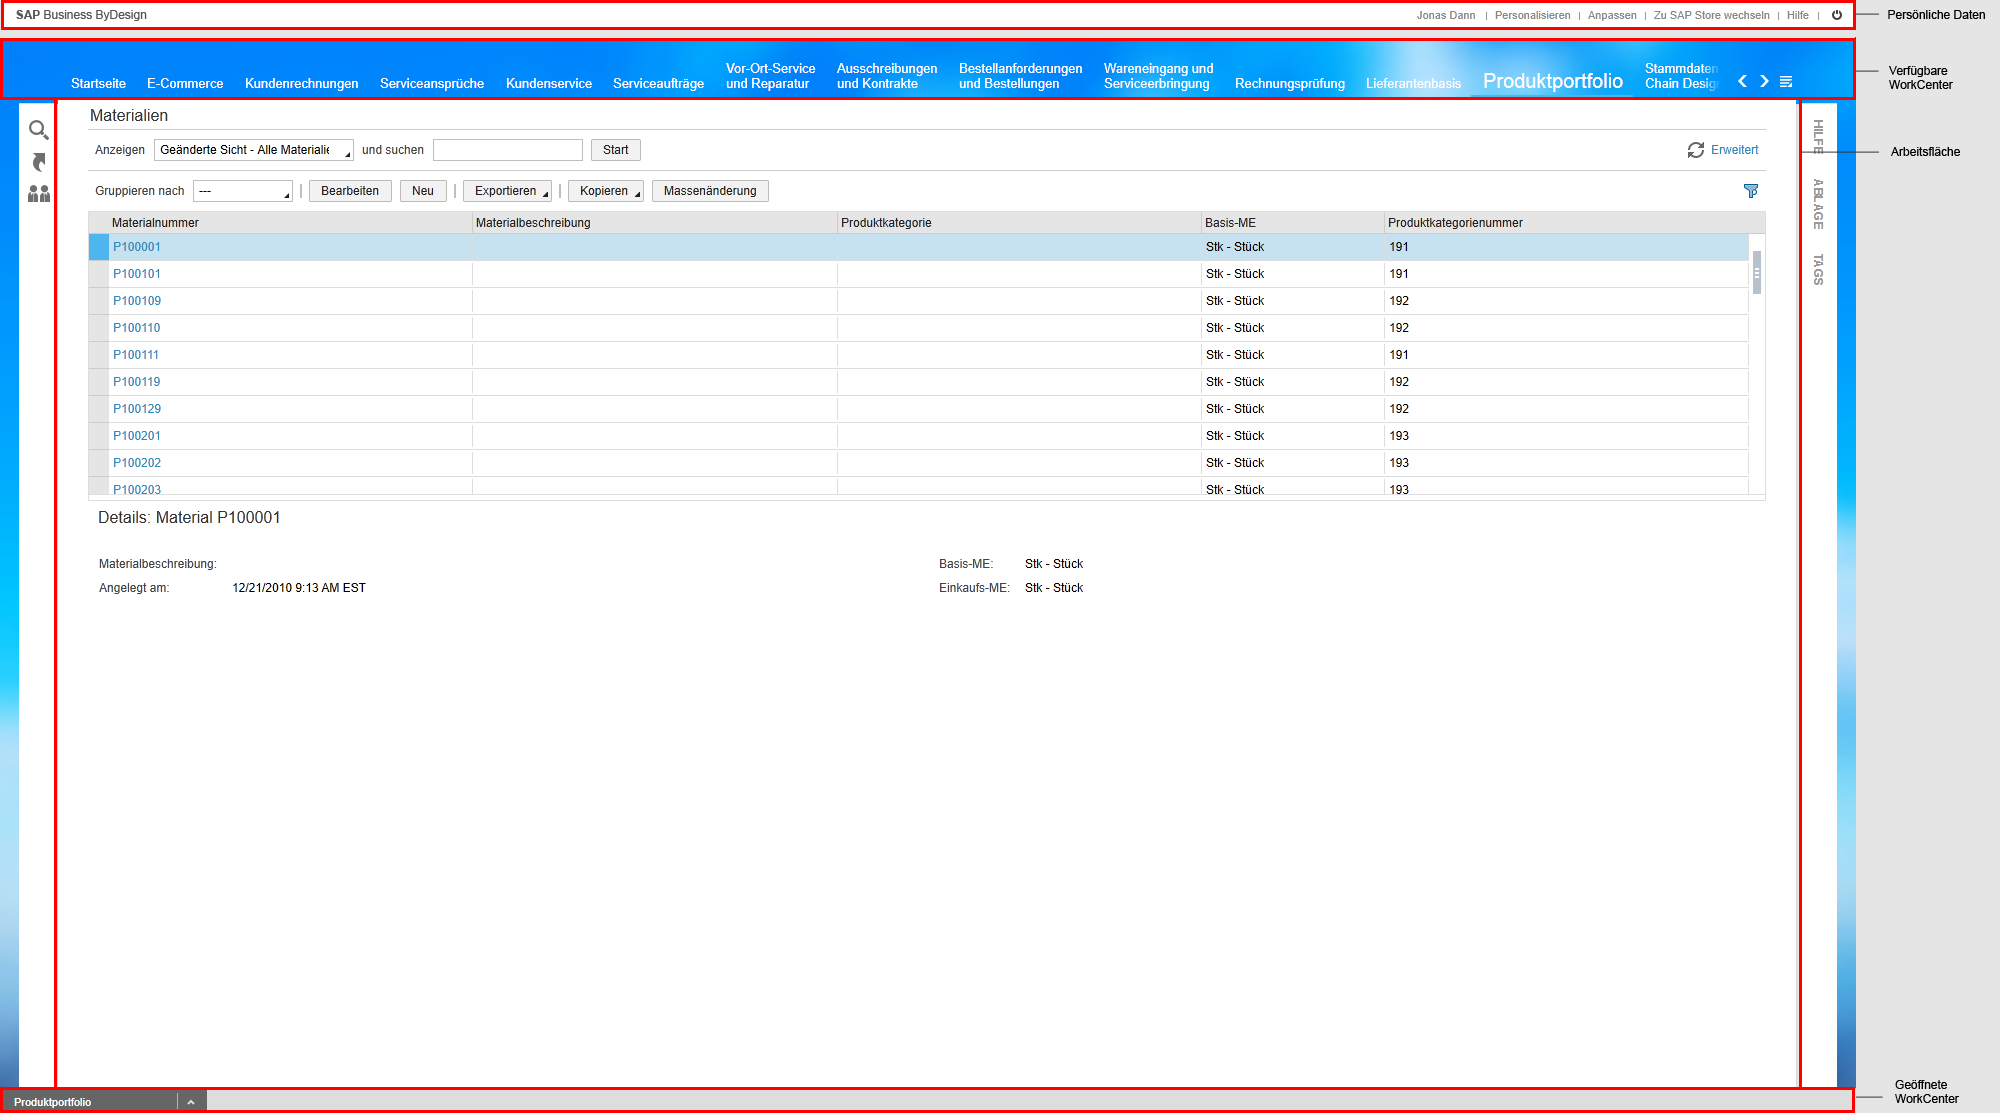
\includegraphics[width=1.0\textwidth]{grafiken/ByDesign-Ubersicht.png}
	\caption{ByDesgin Übersicht}
	\vspace{-10pt}
	\label{abb:byd-overview}
	\end{center}
\end{figure}

\subsubsection{Persönliche Daten}

Hier kann der Mitarbeiter seine Daten, wie \gls{zb} Telefonnummer oder E-Mail, einstellen. Außerdem kann er seinen Benutzeroberfläche in \gls{byd} personalisieren. Weiterhin besteht die Möglichkeit in den \gls{sap}-Store zu wechseln und eine Hilfe aufzurufen.

\subsubsection{Verfügbare WorkCenter}

\gls{byd} ist in verschiedene WorkCenter unterteilt, die jeweils einen Teilgeschäftsprozess abbilden. So kann man \gls{zb} seine Mitarbeiter oder Waren verwalten.

In dieser Sektion der Anzeige kann der User die verschiedenen, für ihn verfügbaren WorkCenter auswählen. Diese werden dann unten im "`Geöffnete WorkCenter"' Bereich angezeigt und in der Arbeitsfläche geöffnet.

\subsubsection{Arbeitsfläche}

Hier werden die eigentlichen Inhalte des Webinterfaces angezeigt. Wenn der Beispielworkflow durchgespielt wird, werden auch nur noch diese Ausschnitte des Bildschirms gezeigt.

\subsubsection{Geöffnete WorkCenter}

Im Bereich "`Geöffnete WorkCenter"' sieht der Mitarbeiter alle WorkCenter, die er im Moment geöffnet hat. Die Anzeige funktioniert wie Tabs in einem Webbrowser und der Nutzer kann damit zwischen verschiedenen Ansichten und Aufgaben wechseln.

%%%%%%%%%%%%%%%%%%%%%%%%%%%%%%
%% KAPITEL Beispielworkflow %%
%%%%%%%%%%%%%%%%%%%%%%%%%%%%%%
%% JONAS                    %%
%%%%%%%%%%%%%%%%%%%%%%%%%%%%%%
\section{Beispielworkflow}

\subsection{Vorstellung des Workflows}
\label{sec:byd-bsp-vorstellung}
% Schulungsworkflow beschreiben (anwendersicht)

\subsubsection{Szenario}

Der Verkaufsbereichsleiter unserer Firma hat auf einer Technologiemesse ein innovatives Produkt entdeckt. Er würde gerne einen neuartigen Solarboiler in das Produktportfolio der Firma aufnehmen. Die Nachfrage nach Innovation und neuen Produkten ist sehr groß.

\subsubsection{Aufgabe des Mitarbeiters}

\begin{enumerate}
 \item Wir müssen in einem Katalog oder elektronischen Marktplatz einen Zulieferer für das gewünschte Produkt finden.
 \item Danach müssen wir den günstigsten Zulieferer finden, der gleichzeitig auch eine hohe Verfügbarkeit gewährleisten kann.
 \item Wenn wir ein passendes Produkt gefunden haben müssen wir dieses in \gls{sap} \gls{byd} einfügen und ihm eine Produktkategorie zuordnen.
 \item Währenddessen müssen alle wichtigen Daten über das Produkt in das System eingepflegt werden.
 \item Nun müssen wir den Zulieferer für das neue Material im \gls{byd} einfügen.
 \item Nachdem wir den Zulieferer angelegt haben können wir ihm jetzt eine Angebotsanforderung schicken.
 \item Zuletzt wird ein Vertrag mit dem Lieferanten geschlossen. 
 \end{enumerate}

\subsection{Umsetzung des Workflows}
\label{sec:byd-bsp-umsetzung}
% technische sicht, "`klickbares"' howto

\subsubsection{Produktsuche}

Im ersten Schritt suchen wir uns ein Produkt und einen Zulieferer auf der Website Alibaba\footnote{\url{alibaba.com}}. Auf dieser Website können kleine Unternehmer ihre Produkte zum Verkauf anbieten. Im Moment sind über 2 Millionen Zulieferer registriert.

Für unser Beispiel verwenden wir den SunSurf SC-IP01\footnote{\url{http://www.alibaba.com/product-detail/SunSurf-SC-IP01-solar-boiler-system_627442099.html?s=p}} Solar Boiler. Dieser kostet zwischen 400 und 500 USD(\$) und muss mindestens zu 15 Stück bestellt werden. Der Zulieferer kann maximal 5000 Stück im Monat liefern.

\subsubsection{Produkt im System anlegen}

Im WorkCenter "`Produktportfolio"' können wir nun die Daten des SunSurf SC-IP01 unter einem neuen Material abspeichern. Dazu klicken wir auf "`Produkte nach Materialien"' und dann auf "`Neu"'. In dem folgenden Formular geben wir nun die Daten des Solar Boilers an (Abbildung \ref{abb:byd-newmaterial}).

Nachdem wir auf "`Sichern und schließen"' geklickt haben wurde unser Material erfolgreich angelegt.

\subsubsection{Zulieferer anlegen}

Im WorkCenter "`Lieferantenbasis"' unter "`Lieferanten"' legen wir jetzt einen neuen Zulieferer an. Dazu klicken wir wieder auf "`Neu"'. In diesem Formular geben wir nun die Daten des Zulieferers ein (Abbildung \ref{abb:byd-newsupplier}).

Nachdem wir auf "`Sichern und schließen"' geklickt haben wurde unser Zulieferer erfolgreich angelegt.

\subsubsection{Angebotsanforderung versenden}

Wir haben jetzt alles vorbereitet um eine Ausschreibung zu erstellen. Dies geschieht im WorkCenter "`Ausschreibungen und Kontrakte"'. Dort gehen wir auf "`Ausschreibungen und Angebote"'. Wir klicken wieder auf "`Neu"' und füllen die allgemeinen Daten für unsere Ausschreibung (Abbildung \ref{abb:byd-rfq-1}). 

Danach können die Produkte hinzugefügt werden, die mit der Ausschreibung behandelt werden sollen (Abbildung \ref{abb:byd-rfq-2}).

Als letztes fügen wir noch die Bieter ein, die dann automatisch über ihre Teilnahme an der Ausschreibung benachrichtigt werden (Abbildung \ref{abb:byd-rfq-3}).

Wenn die Bieter nun Angebote einschicken können wir diese über eine Eingabemaske in \gls{byd} einfügen (Abbildung \ref{abb:byd-rfq-4}). Dabei werden allgemeine Daten und Preise des Anbieters eingegeben (Abbildung \ref{abb:byd-rfq-5}). Weiterhin können wir dann die Angebot anzeigen und vergleichen und dann dem Besten den Zuschlag geben.

\subsubsection{Vertrag schließen}

Nachdem wir dem Angebot nun den Zuschlag gegeben haben können wir den Vertrag prüfen und unser Vorgesetzter kann ihn anschließend annehmen (Abbildung \ref{abb:byd-contract}).

%%%%%%%%%%%%%%%%%%%%%
%% KAPITEL Grenzen %%
%%%%%%%%%%%%%%%%%%%%%
%% JONAS           %%
%%%%%%%%%%%%%%%%%%%%%
\section{Grenzen von ByD}

Trotz der vielseitigen Vorteile von \gls{byd} stößt auch diese Lösung, wie alle anderen, an ihre Grenzen.

\subsubsection{Vordefinierte Geschäftsprozesse}

Durch die Idee hinter \gls{byd}, eine vorkonfigurierte On-Demand Unternehmensmanagement Applikation bereitzustellen, weißt es Nachteile gegenüber den anderen \gls{sme}-Lösungen im Bereich Customizing auf. So kann \gls{byd} nicht beliebig granular konfiguriert werden.

\subsubsection{Module}

Da \gls{byd} in Form von Modulen zusammengestellt wird bekommt der Kunde unausweichlich auch Funktionalität, die er gar nicht benötigt und bezahlt für unnötige Anwendungsbestandteile. In diesem Aspekt sind Business One \ref{sec:business-one} oder \gls{sap} All-in-One \ref{sec:allinone} die bessere Wahl.

\subsubsection{Erweiterbarkeit}

Im Gegensatz zu den beiden anderen \gls{sme}-Systemen kann \gls{byd} nicht beliebig erweitert werden. So können nicht einfach spezifische Prozesse neu entwickelt und in das vorhandene System eingebunden werden, da \gls{byd} keine Möglichkeit bietet eigene Workflows anzulegen und auch \gls{sap} keine weit über die Standardsoftware hinausgehenden Add-Ons anbietet.

